\documentclass[10pt,a4paper]{article}

\usepackage[a4paper,left=1.9cm,right=1.9cm,top=1.5cm,bottom=1.5cm]{geometry}
\usepackage[T1]{fontenc}
\usepackage{lmodern}
\usepackage{graphicx}
\usepackage{booktabs}
\usepackage{tikz}
\usepackage[font=small,labelfont=bf,labelsep=period,skip=4pt]{caption}
\usepackage{enumitem}
\usepackage{needspace}
\usepackage{float}
\usepackage{placeins}
\usepackage{longtable}
\usetikzlibrary{arrows.meta}

\setlength{\parindent}{0pt}
\setlength{\parskip}{4pt}
\setlist{nosep}
\pagestyle{plain}
\sloppy

\newcommand{\screen}[2]{%
  \begin{figure}[H]
    \centering
    \includegraphics[trim=0 230 0 30,clip,width=0.86\textwidth]{../screenshots/#1}
    \caption{#2}
  \end{figure}%
}

\begin{document}

\begin{center}
  {\LARGE\bfseries InvoiceGuard}\\[3pt]
  {\large Accounts Payable Payment Exception and Fraud Prevention}\\[8pt]
  Maadhav\\
  November 2026
\end{center}
\noindent\rule{\linewidth}{0.4pt}

\section{Summary}

InvoiceGuard is an accounts payable control application for Oracle Forms 14.1.2 and Oracle Database. It matches each supplier invoice to its purchase order (PO) and goods receipt (GRN) before payment, and holds invoices that look duplicated, mismatched, tampered with or approved without authority. All rules are PL/SQL packages inside the database. The Forms screens only collect input, call those packages and show the results, so the rules can serve another front end later without being rewritten.

The database layer is verified on Oracle Database 23ai: 70 automated tests pass, all 25 seeded invoices raise their expected holds, and all 17 hold codes fire. The Forms layer compiles with zero errors on Oracle Forms 14.1.2 and runs in a Docker stack (section 6).

\section{Problem}

Accounts payable pays what is billed. Without a check against the purchase order and the goods receipt, a company can pay for goods it never ordered or never received, pay above the agreed price, or pay the same bill twice. The main exposures are:

\begin{itemize}[leftmargin=1.2em,itemsep=2pt]
  \item \textbf{Duplicate invoices:} the same bill entered twice, often with the number written differently, such as INV-01001 and INV1001.
  \item \textbf{Three-way mismatches:} the billed quantity or price differs from the PO or from what was received.
  \item \textbf{Unauthorised approvals:} an invoice approved above the approver's limit, by the person who entered it, or by a user with no approval authority.
  \item \textbf{Bank-detail fraud and split invoices:} a changed remit-to account redirects a payment, and invoices split below an approval tier avoid review.
\end{itemize}

Checking every invoice this way by hand is slow, and the checks become inconsistent as volume grows. Automated three-way matching applies the same rules to every invoice before payment and keeps an audit trail of who approved or released what, and why.

\section{What InvoiceGuard catches}

Each rule raises a hold on the invoice. An invoice with an open hold cannot be approved or paid. Table~\ref{tab:holds} lists the 17 hold codes by category.

\small
\begin{longtable}{@{}l l p{7.3cm} l@{}}
\caption{The 17 hold codes, grouped by category}\label{tab:holds}\\
\toprule
Hold code & Severity & What it checks & Released by \\
\midrule
\endfirsthead
\toprule
Hold code & Severity & What it checks & Released by \\
\midrule
\endhead
    \multicolumn{4}{@{}l}{\textbf{Match} (three-way match against PO and receipt)} \\
    \texttt{PRICE\_VAR} & Medium & Unit price above PO price beyond 2\% and INR 1 per unit & \texttt{AP\_MANAGER} \\
    \texttt{QTY\_REC} & Medium & Billed quantity above net received (received less rejected) & \texttt{AP\_MANAGER} \\
    \texttt{QTY\_ORD} & High & Billed quantity above the quantity ordered on the PO line & \texttt{FIN\_CONTROLLER} \\
    \texttt{NO\_RECEIPT} & Medium & PO line has no goods receipt & \texttt{AP\_MANAGER} \\
    \texttt{AMT\_MISMATCH} & Medium & Header amount differs from lines plus tax by more than INR 1 & \texttt{AP\_MANAGER} \\
    \texttt{PO\_STATUS} & Medium & PO is not open (closed or cancelled) & \texttt{AP\_MANAGER} \\
    \addlinespace
    \multicolumn{4}{@{}l}{\textbf{Duplicate}} \\
    \texttt{DUP\_EXACT} & High & Same vendor and same normalised number as another live invoice & None: cancel the invoice \\
    \texttt{DUP\_SUSPECT} & High & Same vendor and amount within 30 days, or same number and amount at another vendor & \texttt{AP\_MANAGER} \\
    \addlinespace
    \multicolumn{4}{@{}l}{\textbf{Fraud}} \\
    \texttt{PO\_VENDOR} & High & Invoice vendor or PO line does not match the PO & \texttt{FIN\_CONTROLLER} \\
    \texttt{VENDOR\_STATUS} & High & Vendor is inactive or blocked & \texttt{FIN\_CONTROLLER} \\
    \texttt{BANK\_CHANGE} & High & Remit-to account recently changed, not the vendor's active account, or shared with another vendor & \texttt{FIN\_CONTROLLER} \\
    \texttt{DATE\_ANOMALY} & Medium & Invoice dated before its PO, or dated in the future & \texttt{AP\_MANAGER} \\
    \texttt{SPLIT\_SUSPECT} & High & Invoices from one vendor, each just under the INR 500,000 tier, within 7 days, totalling above it & \texttt{FIN\_CONTROLLER} \\
    \texttt{ROUND\_AMT} & Low & Round amount (multiple of 10,000) at or above INR 100,000 & \texttt{AP\_MANAGER} \\
    \addlinespace
    \multicolumn{4}{@{}l}{\textbf{Compliance}} \\
    \texttt{TAX\_VAR} & Low & Tax differs from the PO tax rate applied to the lines by more than INR 1 & \texttt{AP\_MANAGER} \\
    \texttt{GSTIN\_INVALID} & Medium & Vendor GSTIN fails the format or check digit, or does not match the PAN & \texttt{AP\_MANAGER} \\
    \addlinespace
    \multicolumn{4}{@{}l}{\textbf{Authority}} \\
    \texttt{UNAUTH\_APPROVAL} & High & Post-approval scan: approver lacked authority, exceeded the limit, or breached SoD & \texttt{FIN\_CONTROLLER} \\
\bottomrule
\end{longtable}

\textbf{Release rules.} \texttt{FIN\_CONTROLLER} can release any hold that \texttt{AP\_MANAGER} can release. No one can release a hold on an invoice they entered. \texttt{DUP\_EXACT} has no release role: the invoice must be cancelled.

\textbf{Approval controls.}
\begin{itemize}[leftmargin=1.2em,itemsep=2pt]
  \item \textbf{Approval limits.} Each approver has an INR limit set per user. An approval above the limit is refused.
  \item \textbf{Segregation of duties.} The approver cannot be the person who entered the invoice, the PO buyer, or anyone who received goods on that PO.
  \item \textbf{Blocked attempts are logged.} A refused approval is written to the approval history as BLOCKED, even though the transaction is rolled back.
  \item \textbf{Post-approval scan.} A detective check finds approvals made without authority and places an \texttt{UNAUTH\_APPROVAL} hold. That hold blocks payment until a \texttt{FIN\_CONTROLLER} releases it.
  \item \textbf{Locked records.} Approved and paid invoices cannot be changed. The database rejects the change.
\end{itemize}

\section{How it works}

The system uses a thick database and a thin Forms client. Every rule is in an \texttt{IG\_} package in Oracle Database. Each Forms button calls one package procedure and displays the result. Forms never writes the invoice status, the risk score, the approver or the hold rows itself. A replacement front end would call the same packages and get the same answers. Figure~\ref{fig:arch} shows the three tiers.

\begin{figure}[t]
  \centering
  \scalebox{0.9}{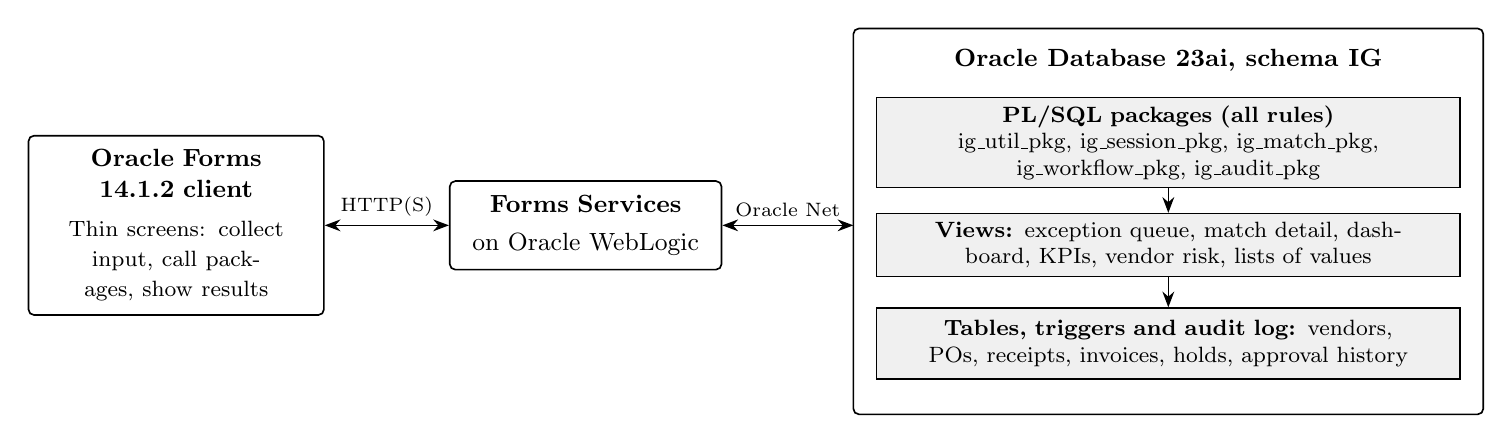
\begin{tikzpicture}[
    blk/.style={draw=black, line width=0.6pt, rounded corners=2pt, align=center, font=\small, inner sep=5pt},
    sub/.style={draw=black, line width=0.5pt, fill=black!6, align=center, font=\footnotesize, inner sep=3pt, text width=7.2cm},
    arr/.style={-{Stealth[length=2mm]}, line width=0.6pt},
    barr/.style={{Stealth[length=2mm]}-{Stealth[length=2mm]}, line width=0.6pt},
    lbl/.style={font=\scriptsize, align=center, fill=white, inner sep=1pt}
  ]
    \node[blk, text width=3.4cm] (cl) at (0,0) {\textbf{Oracle Forms 14.1.2 client}\\[3pt]\footnotesize Thin screens: collect input, call packages, show results};
    \node[blk, text width=3.1cm] (ws) at (5.2,0) {\textbf{Forms Services}\\[3pt]on Oracle WebLogic};
    \draw[barr] (cl) -- node[lbl, above=2pt] {HTTP(S)} (ws);

    \draw[line width=0.6pt, rounded corners=2pt] (8.6,-2.4) rectangle (16.6,2.5);
    \node[font=\small\bfseries] at (12.6,2.1) {Oracle Database 23ai, schema IG};
    \node[sub, minimum height=1.0cm] (pk) at (12.6,1.05) {\textbf{PL/SQL packages (all rules)}\\ig\_util\_pkg, ig\_session\_pkg, ig\_match\_pkg,\\ig\_workflow\_pkg, ig\_audit\_pkg};
    \node[sub, minimum height=0.8cm] (vw) at (12.6,-0.25) {\textbf{Views:} exception queue, match detail, dashboard, KPIs, vendor risk, lists of values};
    \node[sub, minimum height=0.9cm] (tb) at (12.6,-1.5) {\textbf{Tables, triggers and audit log:} vendors, POs, receipts, invoices, holds, approval history};
    \draw[arr] (pk) -- (vw);
    \draw[arr] (vw) -- (tb);

    \draw[barr] (ws.east) -- node[lbl, above=2pt] {Oracle Net} (8.6,0);
  \end{tikzpicture}}
  \caption{Three tiers. All rules run in the database packages. The Forms client and WebLogic only carry requests and results.}
  \label{fig:arch}
\end{figure}

\textbf{Invoice lifecycle.} An invoice starts as \texttt{DRAFT}. Validation moves it to \texttt{ON\_HOLD} if any hold is open, or to \texttt{VALIDATED} if none is. Only a validated invoice can be approved. Editing a validated invoice returns it to \texttt{DRAFT}, so approval always follows a fresh validation. \texttt{APPROVED} and \texttt{PAID} invoices are locked. Figure~\ref{fig:life} shows the states.

\begin{figure}[t]
  \centering
  \scalebox{0.92}{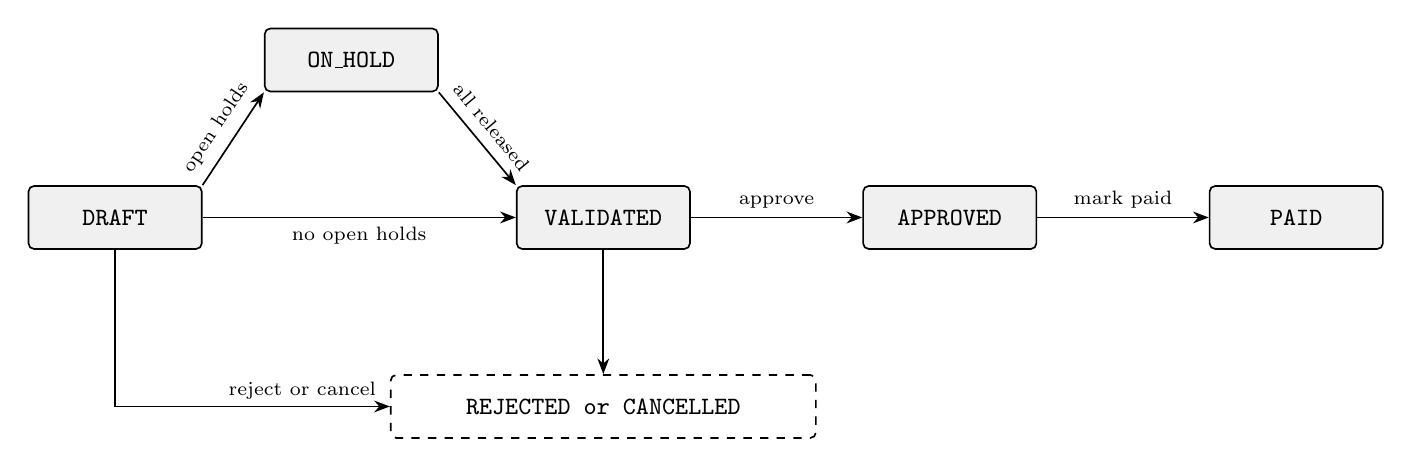
\begin{tikzpicture}[
    st/.style={draw=black, line width=0.6pt, rounded corners=2pt, fill=black!6, font=\small\ttfamily, minimum width=2.2cm, minimum height=0.8cm, inner sep=3pt},
    term/.style={st, dashed, fill=white, minimum width=5.4cm},
    arr/.style={-{Stealth[length=2mm]}, line width=0.6pt},
    lbl/.style={font=\scriptsize, align=center, inner sep=1pt}
  ]
    \node[st] (dr) at (0,0) {DRAFT};
    \node[st] (oh) at (3.0,2.0) {ON\_HOLD};
    \node[st] (va) at (6.2,0) {VALIDATED};
    \node[st] (ap) at (10.6,0) {APPROVED};
    \node[st] (pd) at (15.0,0) {PAID};
    \node[term] (rc) at (6.2,-2.4) {REJECTED or CANCELLED};

    \draw[arr] (dr.north east) -- node[lbl, sloped, above=3pt] {open holds} (oh.south west);
    \draw[arr] (oh.south east) -- node[lbl, sloped, above=3pt] {all released} (va.north west);
    \draw[arr] (dr) -- node[lbl, below=2pt] {no open holds} (va);
    \draw[arr] (va) -- node[lbl, above=2pt] {approve} (ap);
    \draw[arr] (ap) -- node[lbl, above=2pt] {mark paid} (pd);
    \draw[arr] (dr.south) |- (rc.west);
    \node[lbl, anchor=south west] at (1.4,-2.35) {reject or cancel};
    \draw[arr] (va.south) -- (rc.north);
  \end{tikzpicture}}
  \caption{Invoice lifecycle. Validation sends an invoice to ON\_HOLD or VALIDATED. Reject and cancel need a reason. Payment needs an approved invoice with no open holds.}
  \label{fig:life}
\end{figure}

\textbf{Risk score.} Each invoice has a risk score from 0 to 100. It is the sum of the weights of its open holds, plus 10 if the vendor is rated high risk or 5 if medium, capped at 100. Weights range from 5 (\texttt{ROUND\_AMT}) to 60 (\texttt{DUP\_EXACT}). The score is recalculated on every validation, release and scan, so it shows how much is still open on the invoice.


\section{Screens}

The screens below were captured from the running Oracle Forms 14.1.2 client, with the seeded test data. Each image is cropped to the Forms window.

\screen{02_dashboard.png}{Dashboard. KPIs and open holds by hold code, read from the database views.}
\screen{03b_holds_tab.png}{Invoice workbench, Holds tab. SIS-2025-0457 is held as an exact duplicate (DUP\_EXACT, HIGH, risk score 60).}
\screen{04_exceptions_queue.png}{Exception workbench. Open holds across all invoices, with filters, a mandatory release reason and the approval scan.}
\screen{05_blocked_approval.png}{Blocked approval. A clerk's approval is refused by the database (IG-20007) and the attempt is logged as BLOCKED.}

\FloatBarrier
\section{Verification}

\begin{itemize}[leftmargin=1.2em,itemsep=3pt]
  \item \textbf{Database.} On Oracle Database 23ai Free (23.9 image): the schema installs with no invalid objects, and the test suite reports 70 passed and 0 failed.
  \item \textbf{Seeded scenarios.} All 25 seeded invoices land on their expected holds, and all 17 hold codes fire. The expected results are listed in \texttt{db/README\_SCENARIOS.md}.
  \item \textbf{Reports.} All five SQL*Plus reports run with no Oracle errors.
  \item \textbf{Forms compile.} The shared library and all five forms are generated as Forms XML, converted with \texttt{frmxml2f} and compiled with \texttt{frmcmp\_batch}, with zero errors.
  \item \textbf{Forms runtime.} The compiled forms run on Oracle Forms 14.1.2 on WebLogic in Docker. The screens above come from that client.
  \item \textbf{Static checks.} \texttt{forms/tools/check\_refs.py} runs 34 checks with 0 problems: XML structure, package and table references, bind and item names, and item widths against the column definitions.
  \item \textbf{Known gaps.} The custom menu is deferred: \texttt{frmxml2f} rejects every PL/SQL menu item (FRM-31651), so the standard Forms menu and dashboard buttons are used. Row-level severity colours were removed, because a visual-attribute change in POST-QUERY caused a 100 percent CPU loop; severity shows as text. Login is by user name only, which is not authentication.
\end{itemize}

\section{Running it and next steps}

\textbf{Running it.}
\begin{itemize}[leftmargin=1.2em,itemsep=2pt]
  \item \texttt{scripts/db\_up.sh} starts the Oracle Database container, installs the schema and runs the tests. \texttt{scripts/run\_reports.sh} runs the five reports.
  \item \texttt{scripts/forms\_up.sh} is the one command that builds the Forms 14.1.2 stack, compiles the forms and deploys them. It needs the Oracle installers, which the user downloads from Oracle, and the database running.
\end{itemize}

\textbf{Next steps.}
\begin{enumerate}[leftmargin=1.5em,itemsep=2pt]
  \item Build the custom menu module in Forms Builder, and diff its export against our XML.
  \item Restore row-level severity colours in the tabular blocks, without the POST-QUERY loop.
  \item Integrate with Oracle E-Business Suite Payables, so holds and approvals work on live AP invoices through the same packages.
  \item Add a GST e-invoice check that verifies the IRN and QR code. Today InvoiceGuard checks the GSTIN format, its check digit and consistency with the PAN.
  \item Build a web front end that reuses the same \texttt{IG\_} packages, so the rules do not change.
\end{enumerate}

\end{document}
